\documentclass[12pt]{book}

\usepackage[english]{babel}                 %%%%%%%%%%%%%%%%%% (EDIT LANGUAGE)
\usepackage{Styles/Custom}                   %%%%%%%%%%%%%%%%%%    (EDIT NAMES)
\usepackage{AuxiliaryFiles/AuxiliaryFiles}  %%%%%%%%%%%%%%%%%%   (DO NOT EDIT)
\usepackage{Styles/Custom-2}                %%%%%%%%%%%%%%%%%%          (EDIT)

\begin{document}

% Title

\begin{titlepage}
\begin{figure}[ht]\centering
        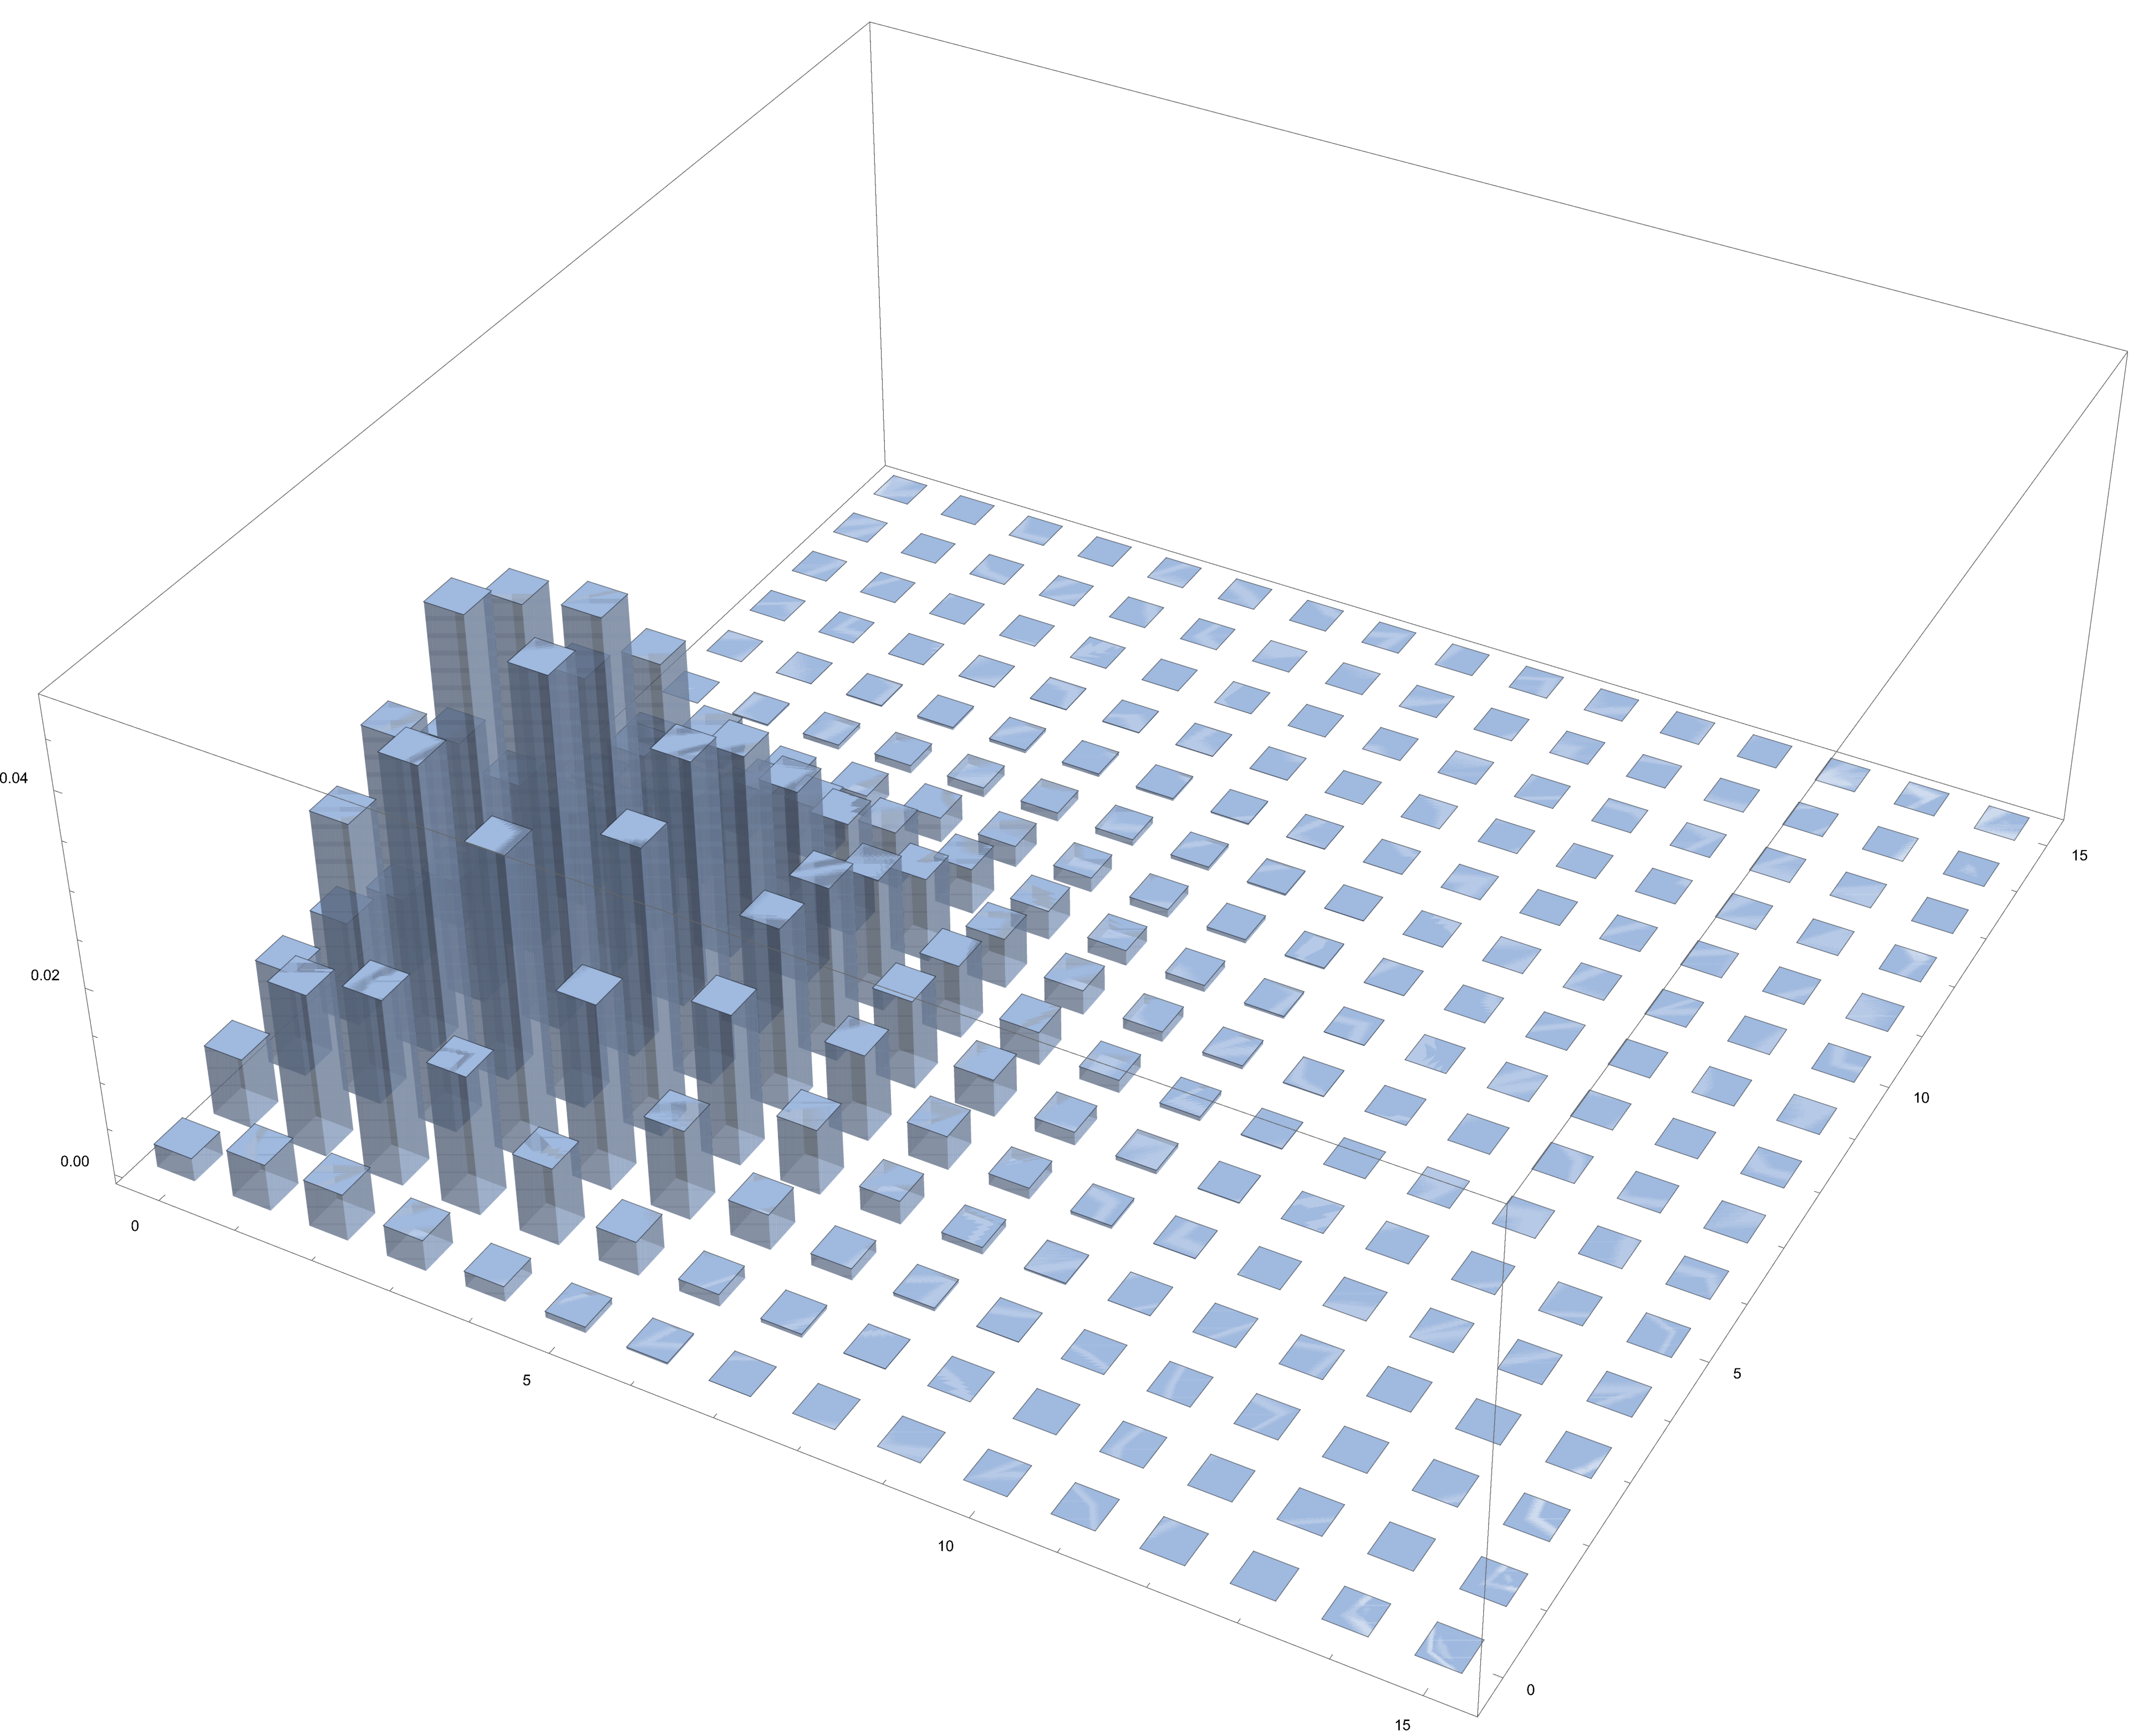
\includegraphics[scale=.15]{Images/Prob2.png}
\end{figure}
\parbox[b]{.95\textwidth}{
    \vspace{1cm}\centering
	{\Huge\bfseries\ Probability and Combinatorics}                          \\[20pt]
	{\large\textit\ The Stochastic Art of Throwing Dice}}
\vfill

\hspace{-.65cm}

\vspace{25pt}
\begin{center}
{\LArge\bfseries\ }              \\[2.5pt]
        {\Large\textsc{Ethan Rubio}                \\[6.5pt]
         \large\textsc{ethan.r.bio@icloud.com}}                       \\[40pt]
\Large\Date
\end{center}
\end{titlepage}

\newcommand\IndexYes{1}
    %   (IF A TABLE OF CONTENTS IS NOT NEEDED, CHANGE 1 TO 0)
\input{AuxiliaryFiles/Frontmatter}  %           (DO NOT EDIT)

% Introduction

\chapter*{}\addcontentsline{toc}{part}{\IntroductionName}
\vspace{-1.5cm}
    \begin{minipage}[r]{.95\textwidth}\raggedleft
    \HUGE\bfseries\IntroductionName
    \end{minipage}
\vspace{2.5cm}

\noindent
         %%%%%%%%%%%%%%%%%%%%%%%%%%%%              (EDIT BELOW)


% Errata

\chapter*{}\addcontentsline{toc}{part}{\ErrataName}
\vspace{-1.5cm}
    \begin{minipage}[r]{.95\textwidth}\raggedleft
    \HUGE\bfseries\ErrataName
    \end{minipage}

\vspace{2.5cm}

\noindent
%%%%%%%%%%%%%%%%%%%%%%%%%%%% EDIT BELOW

\vspace{.5cm}
\begin{longtable}{p{4cm}p{1.45cm}p{8cm}}
	Date & Page&   \\\hline
\Date	& -	& -\\
\end{longtable}


\input{AuxiliaryFiles/Mainmatter}   %%%%%%%%%%%%%%%%%%           (DO NOT EDIT)


\chapter{Foundations of Probability Theory}

\section{Probability Axioms and Conceptual Foundations}

\section{Conditional Probability, Inclusion-Exclusion, and Independence}

\section{Combinatorics and Counting Principles}

\subsection{Permutations and Combinations}

\subsection{Stars and Bars}


\chapter{Random Variables}

\section{Probability Distributions}

\section{Expectation and Variance}

\section{Transformations of Random Variables}

\section{Limit Theorems}

\subsection{Law of Large Numbers}

\subsection{Central Limit Theorem}


\chapter{Advanced Expectation}

\section{Linearity of Expectation}

\section{Indicator Variables}

\section{Coupon Collector Problem}

\section{Markov Chains}

\section{Runs and Sequences}

\section{Random Walks}

\subsection{Gambler's Ruin}

\section{Game Theory and Nim}


\chapter{Advanced Counting Techniques}
\section{Derangements}

\section{Vandermonde's Identity}

\section{Burnside's Lemma}

\section{Distinguisability}

\section{Catalan Numbers}

\section{Generating Functions}

\section{Pigeonhole Principle}

\section{Partitions}

\section{Recurrence Relations}



 \begin{appendices}               %%%%%%%%%%%%%%%%%%    (COMMENT IF NOT NEEDED)
 \input{AuxiliaryFiles/Appendices}    %%%%%%%%%%%%%%%%%%          (DO NOT EDIT)

 %%%%%%%%%%%%%%%%%%%%%%%%%%%%%%%%%%%%%%%%%%%%%%%%%%%%%%%%%%%%%%%%%%%%%%%%%%%%%%%%%%
 \chapter{Title}\label{AppendixA}
 	\blindduck[maths]
 \end{appendices}

% !TEX root = ../BookTemplate.tex
%%%%%%%%%%%%%%%%%%%%%%%%%%%%%%%%%%%%%%%%%%%%%%%%%%%%%%%%%%%%%%%%%%%%%%%%%%%%%%%%%%
\backmatter

%%%%%%%%%                       (BIBLIOGRAPHY PAGE FORMAT)
\fancypagestyle{fancyBibliography}{
	\renewcommand{\headrulewidth}{0.25pt}
	\renewcommand{\footrulewidth}{0.25pt}
	\fancyfoot[LE,RO]{}
	\fancyhead[LO,RE]{\bf\small \BibliographyName}}

%%%%%%%%%%                      (ANALYTIC INDEX PAGE FORMAT)
\fancypagestyle{fancyIndex}{
	\renewcommand{\headrulewidth}{0.25pt}
	\renewcommand{\footrulewidth}{0.25pt}
	\fancyhead[L,R]{}
	\fancyfoot[L,R]{}
	\fancyfoot[C]{\small\thepage}
	\fancyfoot[LE,RO]{}
	\fancyhead[LO,RE]{\bf\small \AnalyticIndexName}}
    %%%%%%%%%%%%%%%%%%          (DO NOT EDIT)
\end{document}